\documentclass[a4paper,notitlepage]{article}
\usepackage{icd-format}
\title{Instrument Control Software (ICS) system architectural design document}
\author{Atsushi Shimono (PFS Software Team)}
\begin{document}

\ICDID{00000}
\ICDREV{001}
\ICDCATEGORY{SOFT / ICS}
\ICDITSIDS{}  % comma separated ID numbers, eg. 1,2,3
\ICDApproval{}
\ICDSuperApproval{}
\ICDChangeRecord{Rev. 001 / First release / 2012--12--10}
\ICDReference{}
\ICDAttachment{}
\icdhead

\section{Abstract}

This document covers system architectural design, especially communication 
architecture among subsystems, for entire ICS. 
As PFS science requirement, the instrument control software shall work 
in collaboration with the targeting software and the on-site data 
reduction pipeline, this document does not touch these interfaces in 
detail.

To prevent future confusions and misunderstandings, 
this design document states definitions of naming, terminology, and 
their covering area, independently from wording at the Subaru.
Also, for ease of communication, relationships to terminologies of local 
standard at the Subaru are presented.

The key words "MUST", "MUST NOT", "REQUIRED", "SHALL", "SHALL NOT", "SHOULD", 
"SHOULD NOT", "RECOMMENDED", and "MAY" in this document are to be interpreted 
as described in [RFC 2119]. 


\section{Software architectural design}

\subsection{Definition of ICS subsystems}

Entire instrument control software will be derivered and work at the 
Subaru Summit Facility (SSF) in cooperation with the Subaru telescope 
control systems.
The entire PFS instrument is consisted of many hardware subsystems 
such as PFI and SpS, and each hardware subsystem will provide its own 
control subsystem. ICS will be consisted of subsystems and shall coordinate 
communications among subsystems well. 
To prevent to have lots of peer to peer connections among subsystems, 
ICS will have one messaging hub system by hub - client typed. 
Every subsystem will have a connection to the messaging hub system, and 
every communication between subsystems should be performed over this system, 
except for large sized and high frequency data transfer connections, such as: 
continuous raw image data transfer per every a few seconds, fiber positioning 
data. 
(Note; also refer Section.~\ref{MHS_Role})
%
In the Subaru telescope control systems (so called SOSS), 
instrument control system which directly connects to the SOSS is called as OBCP
\footnote{What OBCP stands of is not clear, and also its definition varies 
by sentences.} but its naming and role are not clear from instrument 
control point of view.
Here, we define interfaces of our PFS instrument control system to the 
Subaru telescope control system as followings.

\begin{description}
  \item[ICS] Instrument Control System, which includes everything of the 
    PFS instrument control software systems including every subsystem 
    control software. ICS will include any required engineering software 
    including graphical user interfaces, command-line user interfaces, or 
    network data API, but will not include any connected systems at the SSF 
    such as an on-site data reduction pipeline or a targeting software 
    instance. 
  \item[IIC] Instrument Interface and Controller, which has two roles: 
    the only interface of the ICS to the Subaru telescope control system 
    including Gen2, TCS, MLP1 and any other possible candidates; the master 
    controller and sequencer for the entire ICS.
  \item[MHS] Messaging Hub Server, which is the only central communication hub 
    system in entire ICS and every controllable subsystems and environment 
    monitoring systems will connect to this communication hub for sending or 
    recieving commands to peers, sharing status messages, arising operational 
    or environmental alerts, etc.
\end{description}

\subsection{Design as a deployment diagram}

Every subsystem shall be connected directly to the MHS and 
every peer-peer communication should be executed via or transferred by the MHS. 
Each control computing hardware should be connected to one subnet of network 
at the SSF, which is an ethernet network (IEEE 802.3) over metal or optical 
wired, and some of control computing hardware will be required to connect 
some specific network or connection (such as wired serial connection to MLP). 

Deployment diagram for entire PFS ICS is shown in 
figure.~\ref{fig:deploy-diagram}. 

(Note, this section uses deployment diagram, but this does not reflect final 
deployment into computer hardwares.)


\begin{figure}[htb]
  \begin{center}
    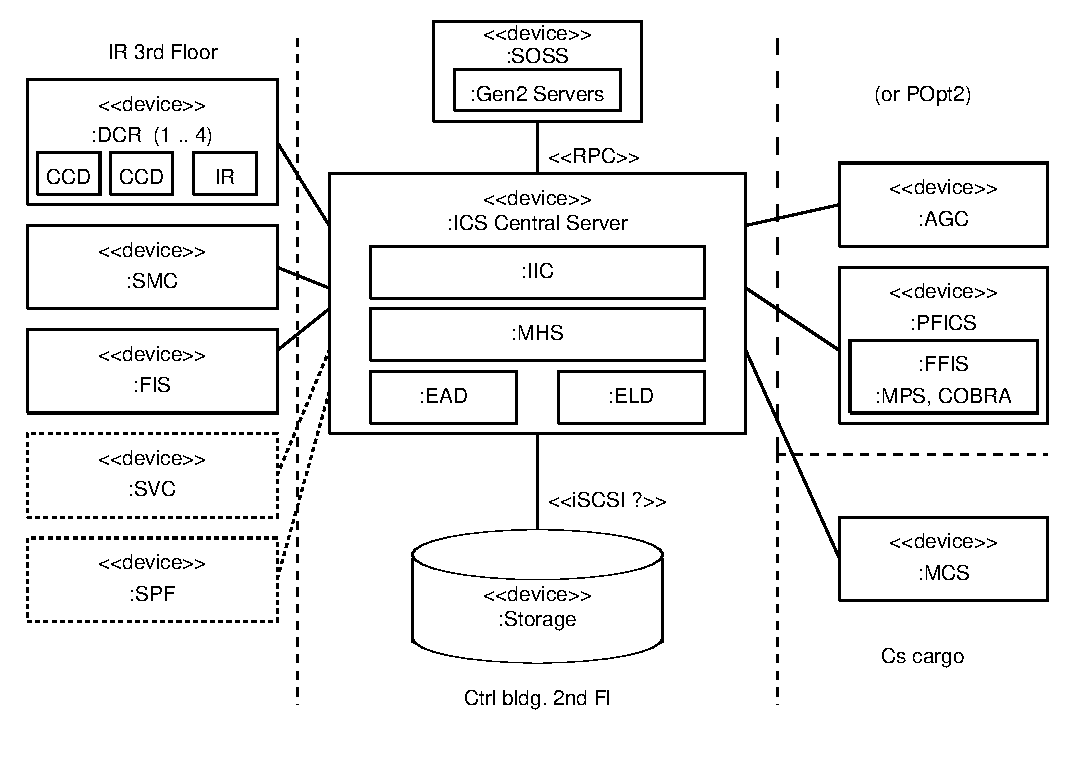
\includegraphics[scale=0.75]{deploy-diagram.eps}
  \end{center}
  \caption{Deployment diagram for entire PFS ICS (Names will change on updates 
          to Section.~\ref{sec:subsystem.def.list})}
  \label{fig:deploy-diagram}
\end{figure}



\subsection{Relation to the Subaru telescope}

Normally, from the Subaru telescope (or SOSS) side, IIC will be visible 
as so called 'OBCP'. Also, except for some required direct connections to MLP 
or TWS, IIC will the only peer from the PFS instrument control software. 

\subsubsection{Communication paths between ICS and SOSS}

To work in coordinate with the Subaru telescope, IIC shall have connections 
to the SOSS by standard procedures defined by the Subaru telescope. 
These procedures and connections are summarized in 
Figure.~\ref{fig:ics-soss-connection}. 

\begin{figure}[htb]
  \begin{center}
    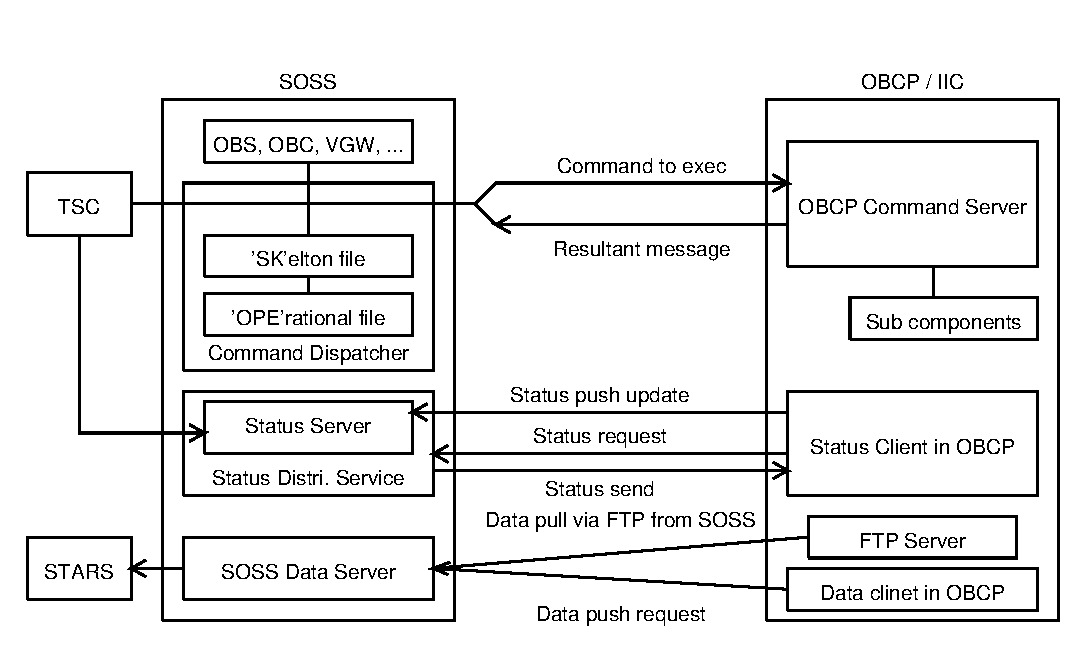
\includegraphics[scale=0.75]{ics-soss-connection.eps}
  \end{center}
  \caption{Connections between SOSS and OBCP. Wordings are of SOSS, not of 
      defined in this document.}
  \label{fig:ics-soss-connection}
\end{figure}

Each connection between SOSS and OBCP means: 

\begin{description}
  \item[Command to exec] One line of text in a format of 'COMMAND NAME=VALUE 
    NAME=VALUE ....' to be executed by the instrument (or any other system 
    controllable from the command dispatcher, including TCS). 
  \item[Resultant message] Result of a command execution including success or 
    not, status message.
  \item[Status push update] Each instrument is required to push its own status 
    to the status server of SOSS when status was changed. This status update 
    shall be triggerd by the instrument side.
  \item[Status request] Each instrument can request to retrieve any status 
    stored in the SOSS status server at any time. Note, the status distriburion 
    service has a matrixed permission table with statuses from which instrument 
    could be sent to which instrument. 
  \item[Status send] The status distribution service will send stored status 
    by request. 
  \item[Data pull via FTP from SOSS] To archive observed or created data, 
    SOSS data server will access a FTP service in each instrument to get 
    a specified file. 
  \item[Data push request] Each instrument shall submit a data push request 
    with a ID specified by SOSS and a file name accessible via FTP, when data 
    is ready to send and be archived. 
\end{description}

\subsubsection{Samples of current sk and ope files}

Since 'sk' and 'ope' files are used in the current SOSS (or Gen2), and we are 
planning to have another mechanism (or protocol), their file formats will not 
directly effect to our software design, but it is important to understand 
how commands will flow into the instrument. 
Both of sk and ope files are dispatched line by line, especially for ope file 
which will be selected by operator or observer line by line. 

Each line in ope files will be like : 

\begin{verbatim}
GETOBJECT EXPTIME=1800 $OBJECT $OBJECT_CONFIG $DEF_IMAG $IMPOS BINNING=3X3
GETBIAS $DEF_IMAG BINNING=3X3
MOVEGUIDE DELTA_RA=0.5 DELTA_DEC=-1.5 $DEF_TOOL
\end{verbatim}

and first word in each line will indicate which sk file to use. (Note, word 
starting with \$ means macro word, and will be translated into pre-defined 
set of words.) 
SOSS will read and execute commands written in each specified sk file, 
which is consisted with lines like :

\begin{verbatim}
Exec K3D WaitExp ;
Exec K3D ChPos MotorName=Mask PositionName=None ;
Exec OBS SetStatus Instrument_Name=K3D Object=$OBJECT ;
Exec OBC QDAS_Display Instrument_name=K3D Input_Frame=!STATOBS.K3D.C1 ;
Exec TSC AG_Tracking Motor=OFF Calc_Region=1 ;
Exec TSC AG Readout=OFF,
Exec VGW Mark_Position V_LAN_DATA=AG Mode=Clear ,
\end{verbatim}

Second word following 'Exec' indicates which instrument (or telescope, 
subsystems in SOSS; in above sample, K3D is the target instrument) 
to send command, and every words following instrument 
indicator will be directly sent to the instrument as a command line 
(including command parameter). Each command parameter is written in name=value 
format, values starting with \$ (operational or pre-defined parameter), or \! 
(SOSS internal working parameter, such as status) will be translated before 
sending to a specified instrument. 

\subsection{Role and capabilities of MHS --- Messaging Hub Server}
\label{MHS_Role}

MHS shall be the only central messaging exchange system for entire PFS 
instrument including every controllable subsystems. 
To coordinate instrument control in a proper way, 
following requirements are applied to a selection of PFS MHS. 

\begin{itemize}
  \item MHS shall be a star-liked message transfer and delivery system, 
    and does not require any (messy) multi-point to multi-point connection.
  \item MHS shall have a capability per each peer to set / select 
    a list of acceptable peers, from which commands shall be accepted and 
    otherwise shall be rejected, as a configuration. 
    This could be implemented at the MHS side or at peers' side as a wrapper 
    layor; both could be accpetable.
  \item MHS shall have a capability to attach external log servers as its 
    peers for every messages through the MHS. 
  \item MHS shuold have a capability to set a 'blocking flag' by each peer 
    to specify peers whose commands shall be acceptable, on demand.
    This flag shall be n-to-n. 
\end{itemize}

For a 'blocking flag', we need to be careful on the system deadlock, 
especially while defining interfaces. 

\subsubsection{Direct communication not using MHS}

Since some communication paths require to transfer huge sized data in high 
frequency, those communication paths (or their data) shall be transferred 
directly between subsystems independent from the MHS. 

For raw image transfer, such as IR up-ramp sampling and AG image, 
subsystems are required to transfer raw observed images (a few MB to a few 
hundreds MB) per every a few seconds. To prevent making throughput down of 
entire MHS and overhead by encodings, 
those raw images shall be transferred directly from 
each generator subsystem to a temporal storage or relay service to the 
Subaru. 
Images from Fiber Quality Monitoring system could be counted in this, 
but Fiber Quality Monitoring system will only be used 
during setup and not observation. Transferring these images may not require 
such high performance and low latency. 

For fiber positioning data, including measured metrology positions' data, 
subsystems are required to work in tight timing budget and their message 
transfer method is also required to be in low latency. 
Also fiber positioning data will be a large number of structured data set 
and will possibly be include some unstructured data, which will require 
each subsystem to handle/encode/decode such large semantic data set. 
This data transfer may be possible to require direct communication between 
hardware subsystems or dedicated database table. 

Every those interface shall be defined as a separated ICD and their brief 
summaries are as followings 
\footnote{We shall update this ICD to include those ICDs in this section 
with brief description.}.

\section{Detailed definition per subsystem}

This section only describes definitions of subsystems. 
Actual interfaces between each subsystem and MHS will be defined as different 
(or separated) ICDs.

\subsection{Controllable subsystems and constraints}
\label{sec:subsystem.def.list}

{\tt 
Note: This section needs to be updated per development of the project. 
Only already well (or somewhat) defined items are shown, and there may be 
many missing items which are in discussion undergoing or not detected yet. 
}

Controllable subsystems within the PFS are: 

\begin{itemize}
  \item PFI (Prime Focus Instrument) part
    \begin{itemize}
      \item Acquisition and Guidance camera (AGC) system
      \item Prime Focus Instrument Control Software (PFICS)
      \item Fiducial fiber back illuminating system (FFIS)
      \item COBRA Positioner Movement Planning Software (MPS)
    \end{itemize}
  \item IR tirtialy floor part, including SpS (Spectrograph System)
    \begin{itemize}
      \item Mechanism Control System for spectrograph
        \begin{itemize}
          \item Shutter mechanisms controller (SHU)
          \item Fiber back illuminating system (BIL)
          \item Dithering Stage (DIS)
          \item Red grating exchange mechanism (REx)
        \end{itemize}
      \item Spectrograph temperature monitoring system
      \item Detector Control System (DCS) for CCDs and IR detectors
      \item Detector temparature sensor and heater system
      \item Vacuum and cryogenic contron system
      \item Fiber Quality Monitoring system
    \end{itemize}
  \item Metrology camera system part
    \begin{itemize}
      \item Metrology camera system (MCS)
    \end{itemize}
\end{itemize}

Also, each subsystem shall have an environment monitoring system to 
measure environment statuses (such as temperatures, humidities, or 
illumination) and to send these statuses to EAD. 

Subsystems required for functionality of IIC and MHS are: 

\begin{itemize}
  \item Environment (Status) archive database (EAD) service
  \item Event logger database (ELD) service
\end{itemize}


Following sections show only well defined subsystems and are not including 
on development or on discussion subsystems. 
Also, for deatiled interface information, find them in each separated ICD. 


\subsubsection{EAD --- Environment and status archive database service}
\paragraph{Definition and subsystem hardware}
EAD does not have any related controllable hardware, and will act as a sub 
service module of IIC. 
EAD will receive status update messages from each environment monitoring 
system of subsystem, archive these statuses with each timestamp 
into its database server, and forward status in the 
required list to the SOSS status server. 
\paragraph{Peers required to communicate}
EAD shall receive any status update message from any environment monitoring 
system, 
and shall forward listed statuses to the SOSS status server. 
\paragraph{Remarks}
EAD will not work on submitting requests of statuses to SOSS from PFS ICS 
including subsystems (via MHS). 

\subsubsection{ELD --- Event logger database service}
\paragraph{Definition and subsystem hardware}
ELD does not have any related controllable hardware, and will act as a sub 
service module of IIC. 
ELD will receive every command through MHS and archive them into database 
server in ELD. 
\paragraph{Peers required to communicate}
ELD shall receive any commands transferred through MHS. 
\paragraph{Remarks}
ELD itself does not have any relationship with other systems (DRP or targeting 
software), but its database server should be accessible from these other 
systems.


\subsection{Activities for one exposure}

For each exposure, following activities will be executed by ICS and its 
subsystems
\footnote{This section is only a sample, and also shows only what is assumed 
by someone (not agreed by full team nor well developed as OCDD / actual 
activity diagram).}.

\begin{itemize}
  \item (IF previous operation/activity was exposure, execute)
  \begin{itemize}
    \item IIC - SHU : Close shutter
    \item IIC - DCS : Readout CCD; Finalize IR detector data
  \end{itemize}
  \item (IF fiber arrangement is required, execute)
  \begin{itemize}
    \item IIC - SHU : Confirm shutter is closed
    \item IIC - BIL : Set blocking flag of BIL (allow control only from PFICS)
    \item IIC - PFICS : Release blocking flag of FFIS
    \item IIC - MCS : Set blocking flag of MCS (allow control only from PFICS)
    \item IIC - PFICS : Execute positioner movement, like
    \begin{itemize}
      \item PFICS - BIL : Confirm operation is allowed
      \item PFICS - FFIS : Confirm illuminator can be turned on
      \item PFICS - MCS : Confirm operation is allowed
      \item Execute loop sequence including MPS, MCS
      \item PFICS - BIL : Release blocking flag
      \item PFICS - MCS : Release blocking flag
    \end{itemize}
  \end{itemize}
  \item IIC - DCS : Confirm data were sent; (Or: Wait readout)
  \item IIC - BIL : Confirm illuminator is off; Set blocking flag of BIL (allow control only from IIC)
  \item IIC - PFICS/FFIS : Confirm FFIS is off; Set blocking flag of FFIS (no turn on)
  \item IIC - DCS : Execute reset (wipe) command
  \item IIC - SHU : Open shutter
  \item (Start exposure)
\end{itemize}





\section{Terminology and References}

\subsection{Abbreviations}

\begin{description}
  \item[AGC] Acquisition and Guidance Camera system
  \item[API] Application Programming Interface
  \item[BIL] Fiber back illuminating system
  \item[CCD] Charge Coupled Device Image Sensor
  \item[CUI] Character-based User Interface
  \item[DCS] Detector Control System for CCDs and IR detectors
  \item[DIS] Dithering Stage
  \item[DRP] Data Reduction Pipeline
  \item[EAD] Environment and status archive database service
  \item[ELD] Event logger database service
  \item[EMS] Environment monitoring systems
  \item[FFIS] Fiducial fiber back illuminating system
  \item[FTP] File Transfer Protocol (RFC 959)
  \item[GUI] Graphical User Interface
  \item[ICD] Interface Control Document
  \item[ICS] Instrument Control Software
  \item[IIC] Instrument Interface and Controller
  \item[IR] InfraRed
  \item[MCS] Metrology Camera System
  \item[MHS] Messaging Hub Server
  \item[MLP] Mid-Level Processor of the Subaru telescope, which is 'sequencer' 
    of Mitsubishi Electric.
  \item[MPS] Movement Planning Software, which will command COBRA positioners.
  \item[PFI] Prime Focus Instrument
  \item[PFICS] Prime Focus Instrument Control Software
  \item[PFS] Prime Focus Spectrograph for the Subaru telescope
  \item[REx] Red grating exchange mechanism
  \item[SHU] Shutter mechanisms controller
  \item[SpS] Spectrograph System
  \item[SSF] Subaru Summit Facility, where entire PFS ICS will be delivered 
    to and will work at.
  \item[TCS] Telescope Control System of the Subaru telescope
\end{description}

\subsection{Applicable or Referenced ICDs}

(nothing listed as for now)

\subsection{References}

\begin{description}
  \item[RFC 2119] Key words for use in RFCs to Indicate Requirement Levels
    (\url{http://www.ietf.org/rfc/rfc2119.txt})
\end{description}


\end{document}

